\section{Gaussian/Linear Discriminant Analysis}

\subsection{Discriminative vs. Generative Models}

  Now we introduce our first example of a generative model, which introduces another division between models (in addition to parametric vs nonparametric, frequentist vs bayesian). Generally, there are two ways to model $\mathbb{P}_{Y \mid X = x}$. 

  \begin{definition}[Discriminative Models]
    \textbf{Discriminative models} attempt to do this directly by  modeling only the conditional probability distribution $\mathbb{P}_{Y \mid X = x}$. We don't care about the underlying distribution of $X$, but rather we just want to try and predict $Y$ given $X$. Essentially, we are trying to approximate the conditional expectation $h(X) = \mathbb{E}[Y \mid X]$, which is the best we can do. Given $X = x$, we use our model of $\mathbb{P}_{Y \mid X = x}$, and our hypothesis function will predict the its mean. 
    \begin{equation}
      h(x) = \mathbb{E}[Y \mid X = x]
    \end{equation}
  \end{definition}

  \begin{definition}[Generative Models]
    \textbf{Generative models} approximate this conditional probability by taking a more general approach. They attempt to model the joint probability distribution $\mathbb{P}_{X \times Y}$ (also called \textbf{inference}), which essentially gives everything we need about the data. Doing this allows us to \textit{generate} more data (hence the name), which may be useful. 
        
    One way to approximate the joint distribution is to model the conditional distribution $\mathbb{P}_{X \mid Y = y}$, which gives the distribution of each labels. Now combined with the probability measure $\mathbb{P}_Y$, we can get the joint distribution. Usually in classification, the $\mathbb{P}_Y$ is easy to approximate (the MLE is simply the fequencies of the labels), so conventionally, modeling $\mathbb{P}_{X \times Y}$ and modeling $\mathbb{P}_{X \mid Y = y}$ are considered the same thing. Once we have these, we can calculate the joint distribution, but in high-dimensional spaces this tends to be computationally hard. Therefore, we usually resort to simply calculating $\mathbb{P}_{X \mid Y = y}$ and then using Bayes rule to approximate 
    \begin{equation}
      \mathbb{P}_{Y \mid X} = \frac{\mathbb{P}_{X \mid Y} \mathbb{P}_Y}{\mathbb{P}_X}
    \end{equation}
    where the normalizing term is computed using Monte Carlo simulations. 
  \end{definition}

  This is the first example of a generative model. In GDA, we basically write the likelihood as 
  \begin{equation}
    \prod_{i=1}^n p(x_i, y_i) = \prod_{i} p(x_i \mid y_i) p(y_i)
  \end{equation}
  where each $p(x_i \mid y_i)$ is Gaussian and $p(y_i)$ is Bernoulli. This specifies $p(x_i, y_i)$ and therefore is called a generative model. In logistic regression, we have 
  \begin{equation}
    \prod_{i=1} p(x_i, y_i) = \bigg( \prod_i p(y_i \mid x_i) \bigg) \bigg( \prod_i p(x_i) \bigg)
  \end{equation}
  and the first term is the logistic function and the second term is unknown. We only use the first part to classify, and this is a discriminative model. You can be agnostic about the data generating process and you can work with less data since there are less things to fit. Some people ask why should you model more unless you have to, so people tend to try to model the minimum, which is why logistic regression is more popular. 

\subsection{Construction}

  GDA assumes that $\mathbb{P}(x\,|y)$ is distributed according to a multivariate Gaussian distribution. Let us assume that the input space is $d$-dimensional and this is a binary classification problem. We set 
  \begin{align*} 
    y & \sim \text{Bernoulli}(\pi) \\
    x\,|\,y = 0 & \sim \mathcal{N}_d (\mu_0, \Sigma) \\
    x\,|\,y = 1 & \sim \mathcal{N}_d (\mu_1, \Sigma)
  \end{align*}
  This method is usually applied using only one covariance matrix $\Sigma$. The distributions are
  \begin{align*}
    p(y) & = \pi^y (1 - \pi)^{1-y} \\
    p(x\,|\,y = 0) & = \frac{1}{(2\pi)^{d/2} |\Sigma|^{1/2}} \exp \bigg(-\frac{1}{2} (x - \mu_0)^T \Sigma^{-1} (x - \mu_0)\bigg) \\
    p(x\,|\,y= 1) & = \frac{1}{(2\pi)^{d/2} |\Sigma|^{1/2}} \exp \bigg(-\frac{1}{2} (x - \mu_1)^T \Sigma^{-1} (x - \mu_1)\bigg)
  \end{align*}
  Now, what we have to do is optimize the distribution parameters $\pi \in (0, 1) \mathbb{R}, \mu_0 \in \mathbb{R}^d, \mu_1 \in \mathbb{R}^d, \Sigma \in \text{Mat}(d \times d, \mathbb{R}) \simeq \mathbb{R}^{d \times d}$ so that we get the best-fit model. Assuming that each sample has been picked independently, this is equal to maximizing 
  \begin{equation}
    L(\pi, \mu_0, \mu_1, \Sigma) = \prod_{i=1}^n \mathbb{P}\big( x^{(i)}, y^{(i)}\,;\, \pi, \mu_0, \mu_1, \Sigma\big)
  \end{equation}
  which is really just the probability that we get precisely all these training samples $(x^{(i)}, y^{(i)})$ given the 4 parameters. This can be done by optimizing its log-likelihood, which is given by 
  \begin{align*}
    l(\pi, \mu_0, \mu_1, \Sigma) & = \log \prod_{i=1}^n \mathbb{P}(x^{(i)}, y^{(i)}; \pi, \mu_0, \mu_1, \Sigma) \\
    & = \log \prod_{i=1}^n \mathbb{P}( x^{(i)} \,|\, y^{(i)}; \mu_0, \mu_1, \Sigma) \, \mathbb{P}(y^{(i)}; \pi) \\
    & = \sum_{i=1}^n \log \bigg( \mathbb{P}( x^{(i)} \,|\, y^{(i)}; \mu_0, \mu_1, \Sigma) \, \mathbb{P}(y^{(i)}; \pi) \bigg)
  \end{align*}
  and therefore gives the maximum likelihood estimate to be 
  \begin{align*}
    \pi & = \frac{1}{N} \sum_{n=1}^N 1\{y^{(n)} = 1\} \\
    \boldsymbol{\mu}_0 & = \frac{\sum_{n=1}^n 1_{\{y^{(n)} = 0 \}} \mathbf{x}^{(n)}}{\sum_{n=1}^N 1_{\{y^{(n)} = 0 \}}} \\
    \boldsymbol{\mu}_1 & = \frac{\sum_{n=1}^n 1_{\{y^{(n)} = 1\}} \mathbf{x}^{(n)}}{\sum_{n=1}^N 1_{\{y^{(n)} = 1 \}}} \\
    \boldsymbol{\Sigma} & = \frac{1}{N} \sum_{n=1}^N (\mathbf{x}^{(n)} - \mu_{y^{(n)}}) (\mathbf{x}^{(n)} - \mu_{Y^{(i)}})^T 
  \end{align*}

  A visual of the algorithm is below, with contours of the two Gaussian distributions, along with the straight line giving the decision boundary at which $\mathbb{P}(y=1\,|\,x) = 0.5$. 
  \begin{figure}[H]
      \centering
      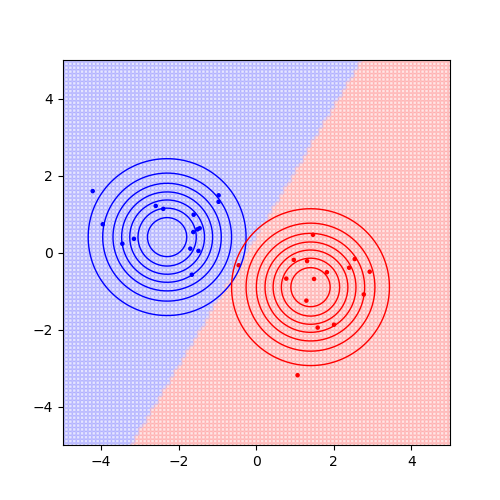
\includegraphics[scale=0.7]{img/GDA.png}
      \caption{GDA of Data Generated from 2 Gaussisans centered at $(-2.3, 0.4)$ and $(1.4, -0.9)$ with unit covariance. The decision boundary is slightly off since MLE approximates the true means. }
      \label{fig:gda}
  \end{figure}

